\begin{figure}[t]
\setlength{\abovecaptionskip}{5pt plus 3pt minus 2pt}
\setlength{\belowcaptionskip}{-20pt plus 3pt minus 2pt}

\centering
\begin{minipage}[b]{0.52\linewidth}
    \centering
    \includegraphics[width=\textwidth,height=3cm]{./images/football_results.pdf}
    \caption{Results on the KTH Multi-view Football II dataset~\cite{footballDS}, in occluded and blurry scenes with dynamic cameras.
    %Motion reconstruction on the KTH Multi-view Football II dataset~\cite{footballDS} in occluded and blurry scenes. 
    %Each row depicts three views of one time frame. 
    %To the right of each image we put a reconstructed rig of the player. % \#20. 
    %The KTH dataset is filmed using moving cameras, hence camera extrinsic parameters vary between frames. 
    %FLEX is ep-free, so it is agnostic to camera parameters and is not affected by the change in their values.
    }
    \label{fig:football_teaser}
\end{minipage}
\hfill
\begin{minipage}[b]{0.44\linewidth}
    \centering
    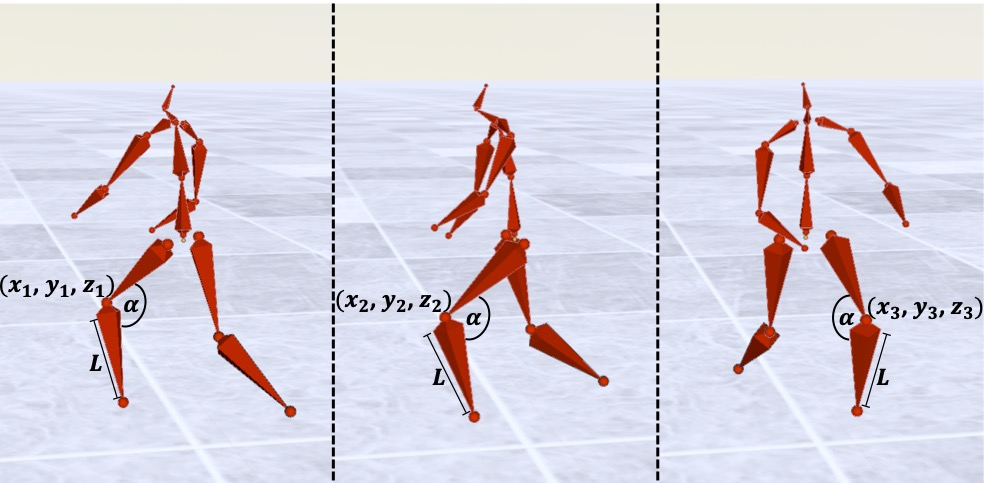
\includegraphics[width=\textwidth,height=3cm]{./images/Skeleton_angles.jpg}
    \caption{3D locations vary across axis systems while 3D rotation angles and bone lengths remain identical.
    %Human rigs observed via the relative axis systems of three cameras. 3D locations vary across axis systems while 3D rotation angles (illustrated with a 2D symbol) and bone lengths remain identical. Thus, fusing the former requires acquaintance of camera parameters while fusing the latter requires none. 
    }
    \label{fig:skeleton_angles}
\end{minipage}
\end{figure}


\sectiontinyvert{Introduction}
Human motion reconstruction is the task of associating a skeleton with
temporally coherent joint locations and rotations. 
Acquiring accurate human motion in a controlled setting, using motion capture systems with adequate sensors is a tedious and expensive procedure that cannot be applied for capturing spontaneous activities, such as sporting events.
%
Motion reconstruction from RGB cameras is low-cost and non-intrusive, but is an uncontrolled setup. Thus, while being simple, it has technical challenges that are worsened by occlusion and depth ambiguity. 
%
Using multiple cameras may alleviate these difficulties as different views may compensate for occlusion and be used for mutual consistency. 
%Yet, exploiting the multi-view setup to improve reconstruction accuracy remains challenging as the relative camera positions may be unknown. 

Recently, there has been a significant progress in using deep learning for pose and motion reconstruction \cite{pavlakos2018ordinal,liu2019improving,sarandi2020metric,shi2020motionet,pavllo20193d,kocabas2020vibe,mehta2020xnect}. Most of these methods work in a monocular setting, but a growing number of works learn a multi-view setting \cite{iskakov2019learnable,tu2020voxelpose,qiu2019cross,he2020epipolar,dong2019fast,rhodin2018learning}. However, these approaches 
%assume that 
\sr{depend on} the 
relative position 
% (translation and rotation) 
between the cameras, derived from extrinsic camera parameters, \sr{and assume they} are given.
%camera parameters are known, and in particular, their relative (extrinsic) positions. 
%
In the lack of extrinsic parameters, several works estimate them~\cite{chu_and_pan_semisupervised,kocabas2019selfsupervised}, 
but at the cost of innate inaccuracy of estimated values.
While camera parameters are often given in multi-view datasets, they are rarely given in dynamic capture environments. We refer to cameras as \emph{dynamic} if they occasionally move during video capture, such that their extrinsic parameters and their inter-camera relative positions are not fixed. \bg{An example of such a camera is the SkyCam~\cite{skycam}, commonly used in sports events.}

% \begin{figure}[thb]
% \centering
% % \includegraphics[width=\linewidth]{./images/Skeleton_cameras.png}
% \includegraphics[width=0.8\linewidth]{./images/teaser cuted.jpg}

% \caption{FLEX reconstructs human motion in environments of multiple cameras, where the camera parameters are unknown.}
% \label{fig:skeleton_cameras}
% \end{figure}

\begin{wrapfigure}{r}{0.3\textwidth}
\setlength{\abovecaptionskip}{-48pt plus 3pt minus 2pt}
\setlength{\belowcaptionskip}{0pt plus 3pt minus 2pt}
\caption*{}

  \centering
    % \includegraphics[width=0.25\textwidth]{./images/teaser cuted.jpg}
    % \includegraphics[width=0.15\textwidth]{./images/teaser cuted more.jpg}
    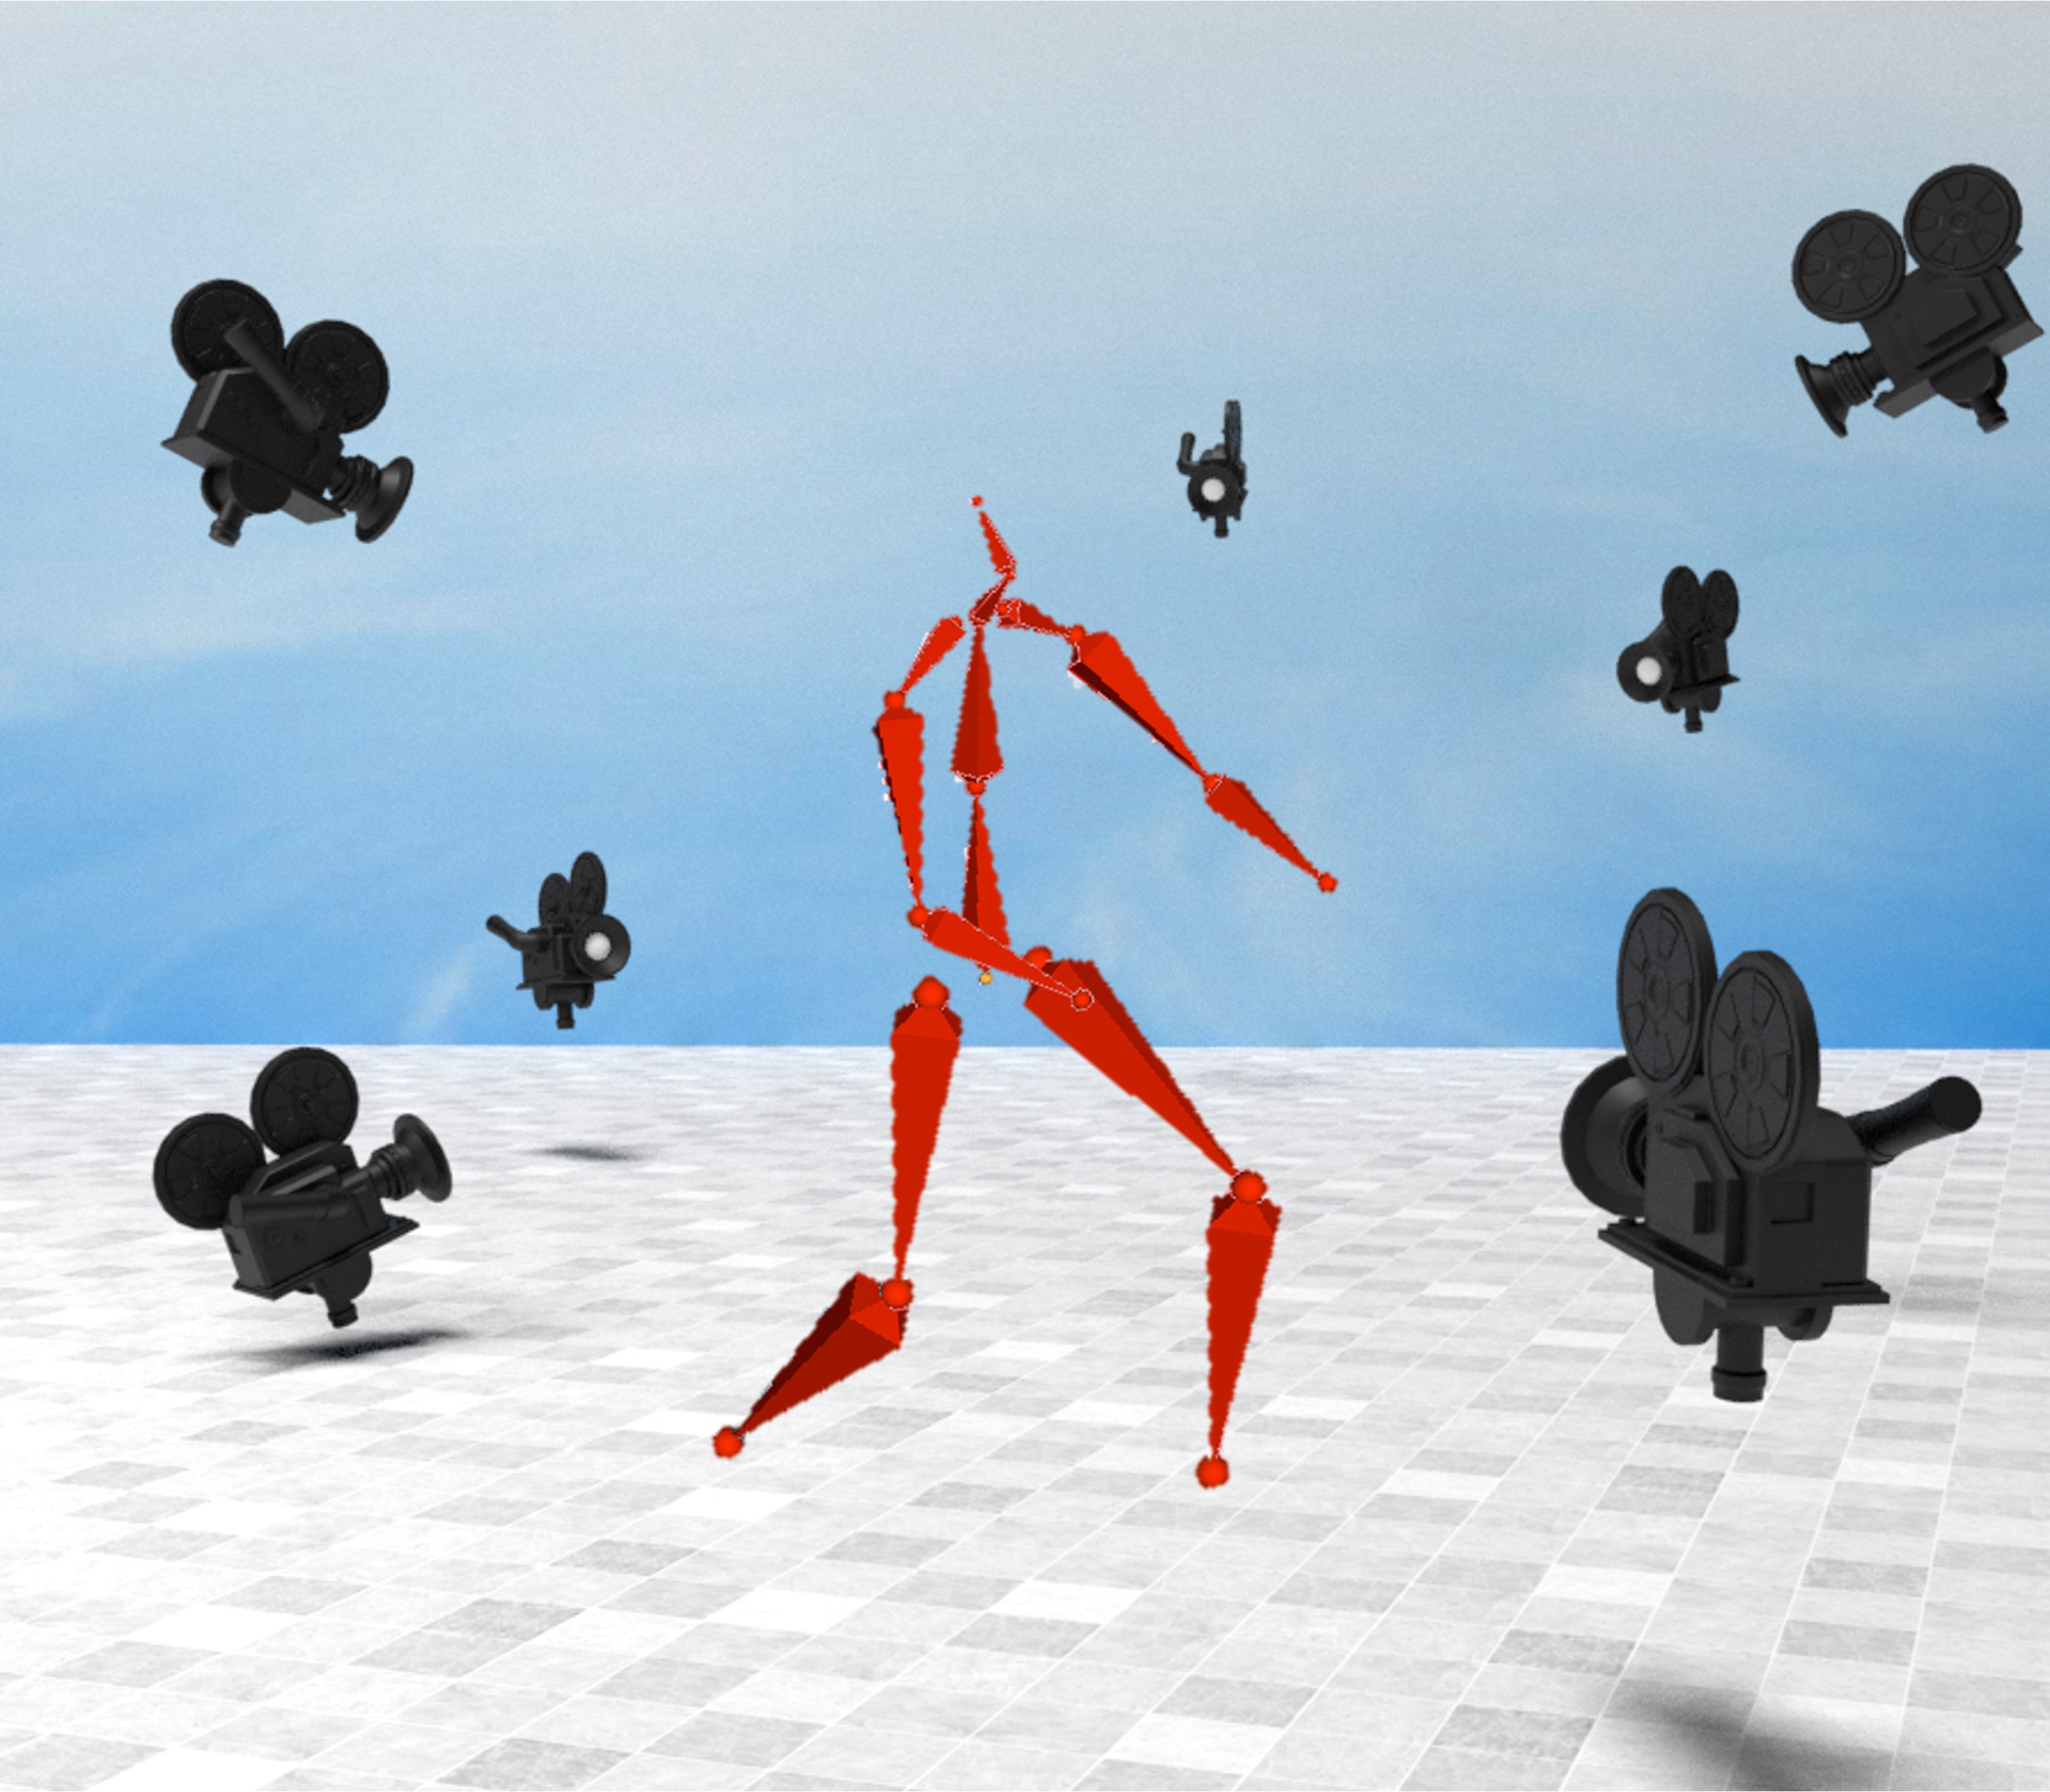
\includegraphics[width=0.3\textwidth]{./images/skeleton_teaser.jpg}
    % \caption{}
%   \caption{FLEX reconstructs human motion in environments of multiple cameras, where the camera parameters are unknown.}
%   \caption{Human motion, captured by multiple cameras.}
   \label{fig:skeleton_cameras}
   
\setlength{\abovecaptionskip}{-45pt plus 3pt minus 2pt}
\setlength{\belowcaptionskip}{-5pt plus 3pt minus 2pt}
\caption*{}
\end{wrapfigure}

%\paragraphtinyvert 
%{ Contribution} 
This work introduces an extrinsic parameter-free (dubbed \emph{ep-free}) multi-view motion reconstruction method, whose setting is illustrated in the inset to the right. 
%
%Our method builds upon a new conceptual observation that uses the common building blocks of joint rotations and bone lengths, to free us from the burdening dependency on the extrinsic parameters of the camera.
Our method builds upon a new conceptual observation that uses the well-known joint rotations and bone lengths, to free us from the burdening dependency on extrinsic camera parameters.
%
Our approach relies on a key insight that joint rotations and bone lengths are identical for all views. 
That is, the 3D angle between skeletal parts is invariant to the camera position.
%
%%%%%%%To exploit this insight, 
We train a neural network to predict 3D joint angles and bone lengths \emph{without} using the extrinsic camera parameters, 
neither in training nor in test time.
Predicting motion rather than locations is not a novel idea by itself. The innovation of our work is in the way we use motion to bypass the need for camera parameters.
The input from multiple cameras is integrated by a novel fusion layer that implicitly promotes joints detected by some cameras and demotes joints detected by others, 
hence  mitigating occlusion and depth ambiguities.

Our model, named FLEX, is an end-to-end deep convolutional network. Its input is multi-view 2D joints that are either given or extracted using a 2D pose estimation technique. 
FLEX employs multi-view blocks with cross-view attention on top of a monocular baseline~\cite{shi2020motionet}, 
and 
%works over a whole video of arbitrary length, embedding temporal information into data features, thus obtaining temporal consistency.
uses temporal information over a video of arbitrary length, thus obtaining temporal consistency.


We evaluate FLEX qualitatively and quantitatively using the Human3.6M~\cite{h36m_pami,IonescuSminchisescu11}, the KTH Multi-view Football II~\cite{footballDS} and the Ski-Pose PTZ-Camera~\cite{ski_ptz} datasets. 
\Cref{fig:football_teaser} demonstrates qualitative results, and more are depicted in \Cref{sec:experiments} and in the \ifarxiv{appendix}\else{supplementary material}\fi.
%
%FLEX is also applied on synthetic videos, generated using Mixamo~\shortcite{mixamo} and Blender~\shortcite{blender}. We have generated these videos to mitigate the lack of a multi-person video dataset that is captured by dynamic cameras, and created them such that they contain severe inter-person occlusions.
FLEX is also applied on synthetic videos. We have generated these videos using Mixamo~\shortcite{mixamo} and Blender~\shortcite{blender},  to mitigate the lack of a multi-person video dataset that is captured by dynamic cameras, and created them such that they contain severe inter-person occlusions.

We compare performance with state-of-the-art methods that are not ep-free and show comparable results. To simulate an ep-free setting, we perturb ground-truth camera parameters or use works that estimate them. We show that in an ep-free setting, our model outperforms state-of-the-art by a large margin. 

Our main contributions are twofold: (i) a network that reconstructs motion and pose in a multi-view setting with unknown extrinsic camera parameters, and (ii) a novel fusion layer with a multi-view convolutional layer combined with a multi-head attention mechanism over a number of views.
